\section{Auswertung}
\subsection{Magnetfeld von Spulen}
\subsubsection{Kurze Spule}
\label{sec:1}
In diesem Abschnitt wird die gemessene Magnetfeldstärke auf der radialsymetrischen 
Achse von einmal einer kleinen und einer großen Spule mit den theoretischen Werten für die 
erwartete Magnetfeldstärke verglichen? 
\begin{table}[H]
    \centering
    \caption{Messwerte der kleinen Spule.}
    \label{tab:t1}
    %\sisetup{table-format=1.1, per-mode=reciprocal}
    \begin{tblr}{
        colspec = {S S},
        row{1} = {guard, mode=math},
      }
      \toprule
      x (\unit{\centi\meter}) & Magnetfeldstärke (\unit{\tesla}) \\
      \midrule
      0   &0.083\\
      1   &0.112\\
      2   &0.154\\
      3   &0.230\\
      4   &0.399\\
      5   &0.727\\
      6   &1.282\\
      7   &1.703\\
      8   &2.053\\
      9   &2.105\\
      10  &1.981\\
      11  &1.589\\
      12  &1.029\\
      13  &0.558\\
      14  &0.332\\
      15  &0.192\\
      16  &0.126\\
      \bottomrule
    \end{tblr}
\end{table}
\autoref{tab:t1} sind die aufgenommenen Messwerte der Magnetfeldstärke auf der Achse 
der kleinen Spule zu entnehmen. x ist der Abstand von einem Punkt aus, welcher 5 \unit{\centi\meter} von 
der Spule entfernt liegt, durch die Spule durch bis 5 \unit{\centi\meter} aus der Spule herraus. Des weiteren 
sind die Messwerte in \autoref{fig:1} graphisch dargestellt.
\begin{figure}
    \caption{Magnetische Feldstärke kleine Spule}
    \label{fig:1}
    \centering
    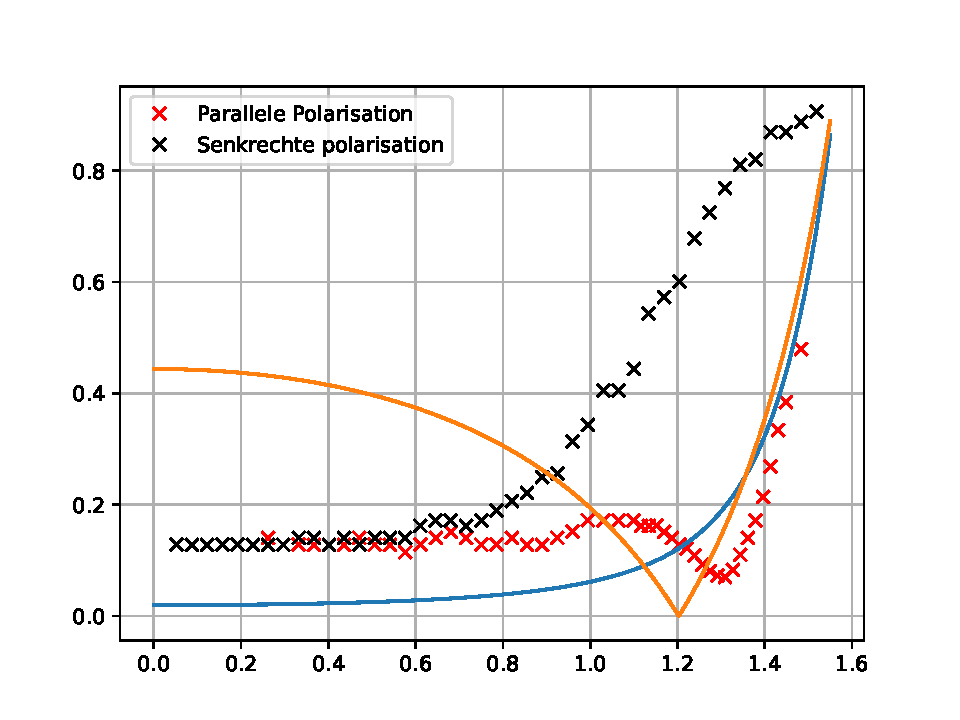
\includegraphics{"build/plot.pdf"}
\end{figure}
Wenn man bedenkt, dass der eintrit der Hall sonde in das Magnetfeld fünf \unit{\centi\meter} 
von $x = 0$ entfernt liegt und auch nach dem Austritt $5$ weitere Messwerte aufgenommen wurden, 
kann man die restlichen Messwerte, die in der Spule aufgenommen, Mitteln um das Magnetfeld im 
innern der Spule zu berechnen. Damit kommt man zu einer Feldstärke von 
\begin{equation*}
    \symbf{B}_{exp} = \qty{1.63(0.18)}{\tesla}.
\end{equation*}
Die Theoretische Magnetfeldstärke im inneren der Spule kann mit \autoref{eqn:4} Bestimmt werden.
Mit den Werten $ I = 1\unit{\ampere}$,$ n = 100 $ und einer Länge von ca 8\unit{\centi\meter}
ergibt sich 
\begin{equation*}
    \symbf{B}_{theo} = \qty{1.57e-3}{\tesla} = \qty{1.57}{\milli\tesla}
\end{equation*}

\subsubsection{Lange Spule}
Bei der Ermittlung der Magnetfeldstärke in der Langen Spule wird genauso verfahren, wie schon 
in \autoref{sec:1}.
\label{sec:Auswertung}

